%++++++++++++++++++++++++++++++++++++++++
% Don't modify this section unless you know what you're doing!
\documentclass[letterpaper,12pt]{article}
\usepackage{tabularx} % extra features for tabular environment
\usepackage{amsmath}  % improve math presentation
\usepackage{graphicx} % takes care of graphic including machinery
\usepackage[margin=1in,letterpaper]{geometry} % decreases margins
\usepackage{cite} % takes care of citations
\usepackage[final]{hyperref} % adds hyper links inside the generated pdf file
\hypersetup{
	colorlinks=true,       % false: boxed links; true: colored links
	linkcolor=blue,        % color of internal links
	citecolor=blue,        % color of links to bibliography
	filecolor=magenta,     % color of file links
	urlcolor=blue         
}
%++++++++++++++++++++++++++++++++++++++++


\begin{document}

\title{6.815 Problem Set 10}
\author{Casey Hong}
\date{\today}
\maketitle

\section{Introduction}
For this assignment I chose to reproduce Salavon-style algorithmic art. Specifically, I tried to recreate his color wheel piece and atmospheric amalgamations. I selected this project because I really enjoyed reproducing the Sergey Prokudin-Gorsky photographs earlier in the course, and felt that this would be similarly rewarding.

\section{Background}
In this section I summarize three related papers.

\subsection{AverageExplorer: Interactive Exploration and Alignment of Visual Data Collections}
This paper by Jun-Yan Zhu, Yong Jae Lee, and Alexei Efros (2014) presents an interactive framework for visualizing weighted mean averages of image collections. The authors find that it is hard to recreate Salavon's images from automatically scraped images from the web because the data is too varied, so they create a user interface for user-guided alignment. Different brush tools allow the user to specify regions or features to sharpen or emphasize in the average, and the images in the ``image stack" are then warped for proper alignment.

\subsection{Scene Completion Using Millions of Photographs}
This paper by James Hays and Alexei Efros (2007) presents a method for inpainting, or image completion, using a very large internet database (scraped from Flickr). They do a two-stage search in which the first stage finds semantically similar images and the second stage finds images with patches that match the area surrounding the missing region. They use Poisson blending and graph-cut segmentation to minimize blending artifacts. 

\subsection{What Makes Paris Look Like Paris?}
This paper by Carl Doersch, Saurabh Singh, Abhinav Gupta, Josef Sivic, and Alexei Efros (2012) presents a method to automatically find visual elements that are most distinctive for a certain region (e.g. Paris). While Salavon's amalgamations are not as computer vision oriented, they similarly try to visually express geographically-informative features in a more atmospheric way. The proposed method scrapes tens of thousands of geo-localized images from Google Street View (preferred over Flickr due to Flickr's bias for tourist-y landmarks) and searches for geographically discriminative features in the images via an iterative clustering algorithm.

\section{Algorithm}
In this section I describe the algorithms used for the project. The image manipulations were very straightforward; the two most significant algorithms that were applied were the planet projection used for the color wheel and the mean-averaging used for the amalgamations. The planet projection computes for each pixel the corresponding polar coordinates, mapping the bottom of the input to the center of the output, and the top of the input to the outer edge edge. With the flat rectangular color wheel as input, we can apply this algorithm to map each pixel to the radial output in order to achieve the wheel effect. For the amalgamations, the output is simply a mean-average of all the input pixels.

\section{Procedure}
The implementation of this project consisted of two phases: first, setting up a mechanism to query and retrieve images from Flickr, and second, applying some simple image processing algorithms to recreate the color wheel and amalgamation effects. In the first phase, I made use of several outside libraries (curlcpp and jsoncpp) to query Flickr for images that matched a given search term. Because the images are downloaded as jpeg, I used ImageMagick's Magick\raisebox{.3\height}{\scalebox{.7}{+}}\raisebox{.3\height}{\scalebox{.7}{+}} library to convert to png. Getting the outside libraries to compile was a bit of a nightmare due to my limited experience with Makefiles and interfacing with the web in C++ in general. I also found that the Flickr results frequently did not cooperate with Magick\raisebox{.3\height}{\scalebox{.7}{+}}\raisebox{.3\height}{\scalebox{.7}{+}}'s conversion process (more on how this affected the resulting images in the next section). In the second phase, I did some fairly straightforward image processing to recreate Salavon's algorithmic art as described in the previous section.

\section{Results} 

\subsection{Color Wheel}
\begin{figure}
	\centering
	\includegraphics[scale=0.04]{../Output/colorWheel.png}
	\caption{Flat rectangular version of the ROYGBIV color wheel.}
\end{figure}
Figure 1 shows the flat rectangular version of the color wheel. Figure 2 shows some visualizations of intermediate steps of the procedure, giving us a closer look at some of the details in the mosaicking process. For example, notice on the left of Figure 2 that some of the results returned for ``red,orange" are images of items that are small and red with a more prominently non-red background (e.g. the ladybug or rose). Also notice that on the right of Figure 2 that empty black tiles can arise in the case of a failed jpeg-to-png conversion. In Figure 3 I show the circular version of the color wheel, created by applying the pano2planet stereographic projection from pset 7 to a flat rectangular input. In Figure 4 I show my attempt at a more traditional mosaic; the turtle painting to the left is the reference, and the result is to the right.

\begin{figure}
	\centering
	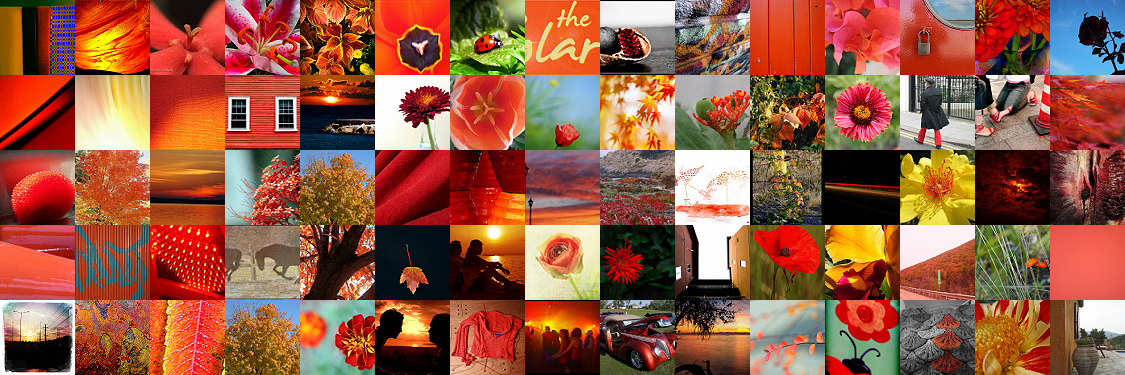
\includegraphics[scale=0.15]{../Output/red,orangeAggregate.png}
	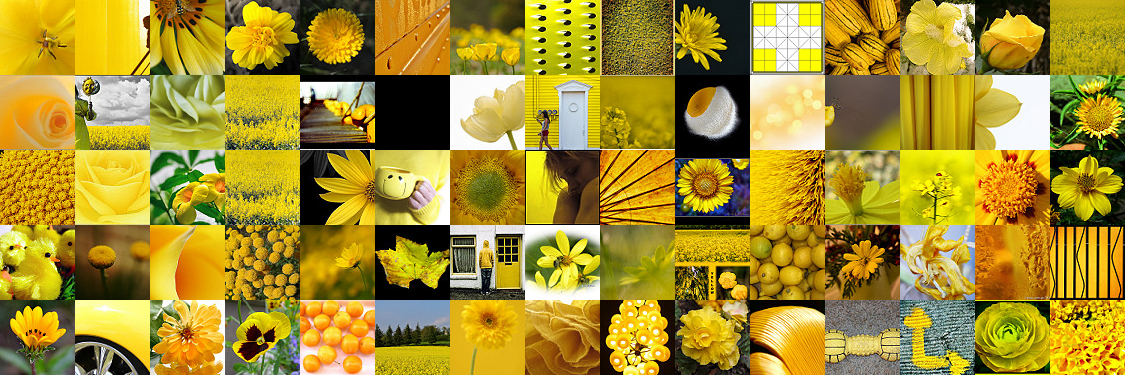
\includegraphics[scale=0.15]{../Output/yellowAggregate.png}
	\caption{Intermediate mosaic results for a single color query.}
\end{figure}
\begin{figure}
	\centering
	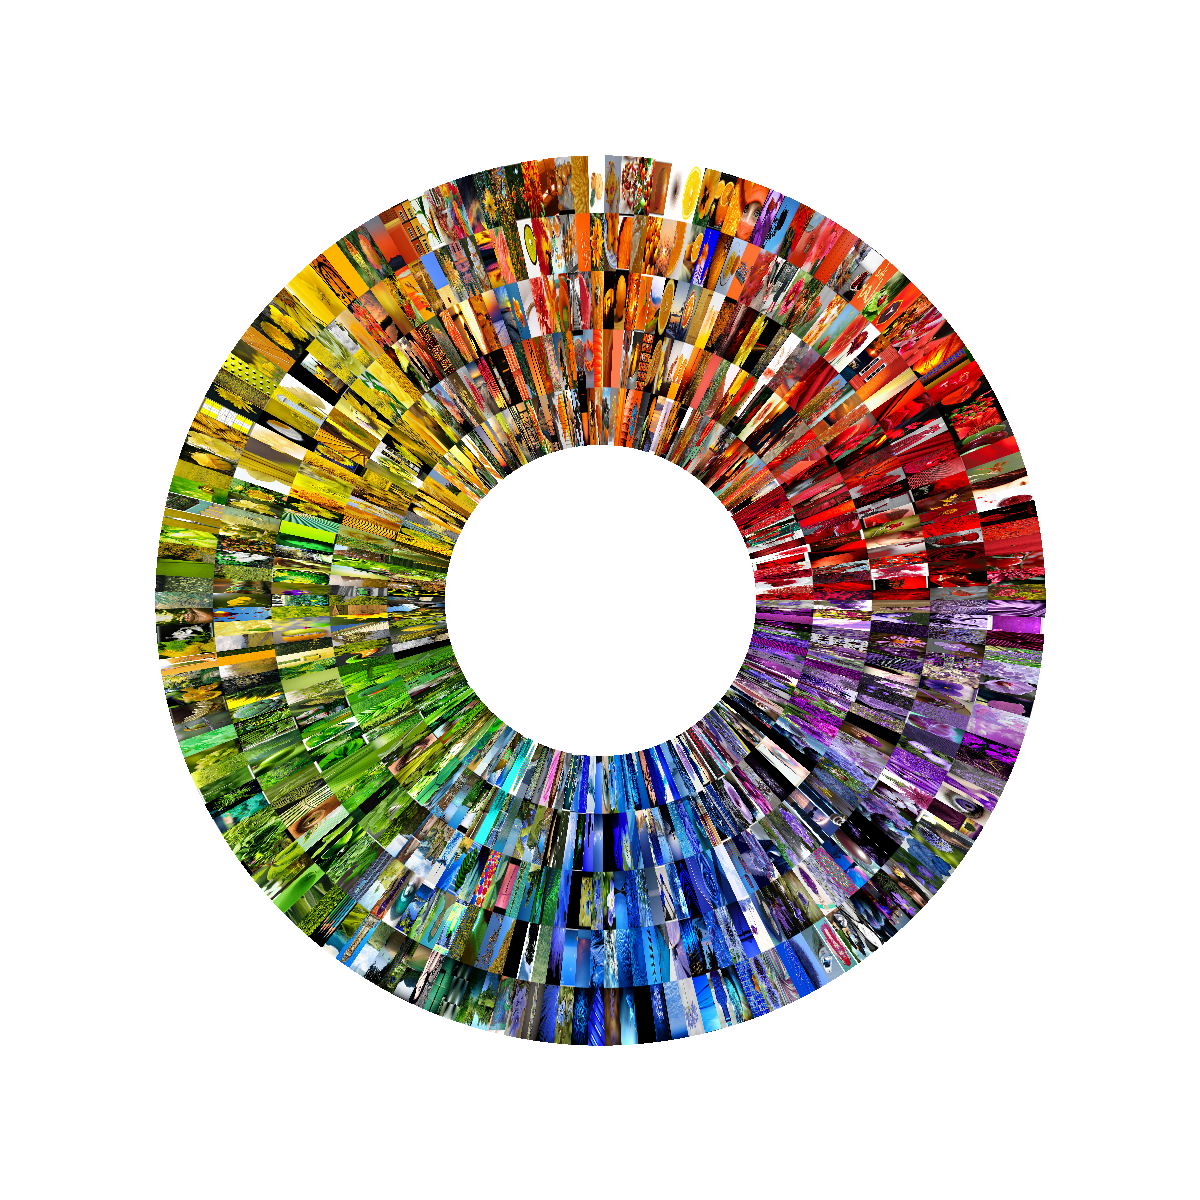
\includegraphics[scale=0.2]{../Output/colorWheel-2.png}
	\caption{The circular version of the color wheel.}
\end{figure}

\begin{figure}
	\centering
	\includegraphics[scale=0.0613]{../Input/turtle.png}
	\includegraphics[scale=0.06]{../Output/turtleMosaic.png}
	\caption{An attempt at a more traditional mosaic result.}
\end{figure}

\subsection{Amalgamations}
Figure 5 shows amalgamations of some mountains. The top left is an amalgamation of 52 images of Half Dome; the top right is one of 30 images of Mt. Rainier, the bottom left is of 22 images of Mt. Denali, and the bottom right is of 34 images of Mt. Everest. It is interesting to note how much bluer the Half Dome and Everest amalgamations are compared to the ones of Mt. Rainier and Mt. Denali. For fun I also did amalgamations of 4 U.S. cities (NYC, Boston, Seattle, and Chicago) and 2 international cities (Seoul and Paris) and show the results in Figure 6.

\begin{figure}
	\centering
	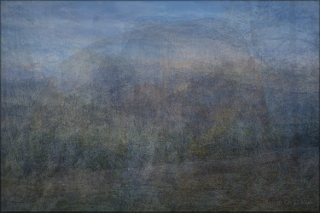
\includegraphics[scale=0.4]{../Output/hd-amalgamation.png}
	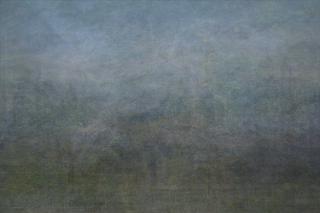
\includegraphics[scale=0.4]{../Output/rainier-amalgamation.png} \\
	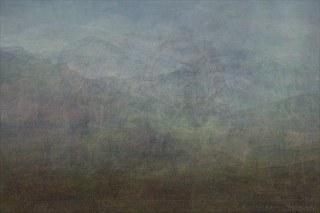
\includegraphics[scale=0.4]{../Output/denali-amalgamation.png}
	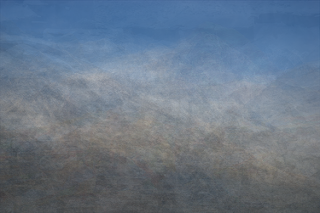
\includegraphics[scale=0.4]{../Output/everest-amalgamation.png}
	\caption{Top row: Half Dome and Mt. Rainier. Bottom row: Mt. Denali and Everest.}
\end{figure}

\begin{figure}
	\centering
	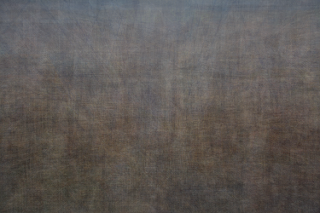
\includegraphics[scale=0.4]{../Output/nyc-amalgamation.png}
	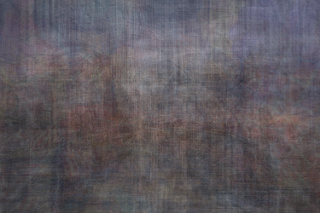
\includegraphics[scale=0.4]{../Output/boston-amalgamation.png}
	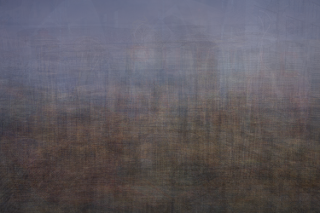
\includegraphics[scale=0.4]{../Output/seattle-amalgamation.png}
	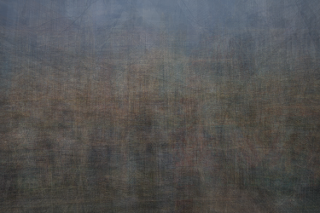
\includegraphics[scale=0.4]{../Output/chicago-amalgamation.png}
	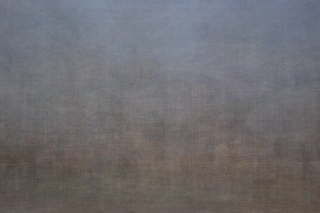
\includegraphics[scale=0.4]{../Output/seoul-amalgamation.png}
	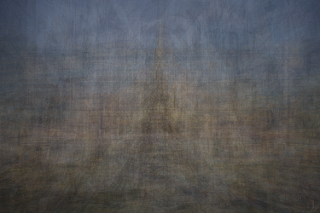
\includegraphics[scale=0.4]{../Output/paris-amalgamation.png}
	\caption{Top row: New York, Boston, Seattle. Bottom row: Chicago, Seoul, Paris. I was pleased to see that the Eiffel tower is somewhat visible in the Paris amalgamation, and was also a little surprised that the Seattle amalgamation turned out to be more blue than gray.}
\end{figure}


\end{document}
